%%%%%%%%%%%%%%%%%%%%%%%%%%%%%%%%%%%%%%%%%
% Master Template Latex Buku  
% Last edited : 23 Juni 2019 
%
% Important note:
% Chapter heading images should have a 2:1 width:height ratio,
% e.g. 920px width and 460px height.
%
% The original template (the Legrand Orange Book Template) can be found here --> http://www.latextemplates.com/template/the-legrand-orange-book
%
% Original author of the Legrand Orange Book Template:
% Mathias Legrand (legrand.mathias@gmail.com) with modifications by:
% Vel (vel@latextemplates.com)
%
% Original License:
% CC BY-NC-SA 3.0 (http://creativecommons.org/licenses/by-nc-sa/3.0/)
%%%%%%%%%%%%%%%%%%%%%%%%%%%%%%%%%%%%%%%%%
 
%----------------------------------------------------------------------------------------
%	PACKAGES AND OTHER DOCUMENT CONFIGURATIONS
%----------------------------------------------------------------------------------------

\documentclass[a4paper,
12pt, %font size default
fleqn, %left-justified equations
]{book}

%Definisi author dan judul buku
\title{Pemrograman dan Komputasi Numerik}
\author{Sholihun-Zohan Syah Fatomi}
\date{\today}

%\usepackage[top=3cm,bottom=3cm,left=3.2cm,right=3.2cm,headsep=10pt,letterpaper]{geometry} % Page margins
\usepackage[top=3cm,bottom=3cm,left=4cm,right=3cm,headsep=8pt,a4paper]{geometry} % Page margins

\usepackage{xcolor} % Required for specifying colors by name
%\definecolor{ocre}{RGB}{210,105,30} % Define the orange color used for highlighting throughout the book
\definecolor{ocre}{RGB}{0,0,0}

% Font Settings
\usepackage{avant} % Use the Avantgarde font for headings
%\usepackage{times} % Use the Times font for headings
\usepackage{mathptmx} % Use the Adobe Times Roman as the default text font together with math symbols from the Sym­bol, Chancery and Com­puter Modern fonts

\usepackage{microtype} % Slightly tweak font spacing for aesthetics
\usepackage[utf8]{inputenc} % Required for including letters with accents
\usepackage[T1]{fontenc} % Use 8-bit encoding that has 256 glyphs
\usepackage{xcolor}

% Bibliography
%\usepackage[style=alphabetic,sorting=nyt,sortcites=true,autopunct=true,babel=hyphen,hyperref=true,abbreviate=false,backref=true,backend=biber]{biblatex}
%\addbibresource{bibliography.bib} % BibTeX bibliography file
\RequirePackage{natbib}
\bibliographystyle{humannat} %format daftar pustaka
%\defbibheading{bibempty}{}


%%%%%%%%%%%%%%%%%%%%%%%%%%%%%%%%%%%%%%%%%
% This is based on the Legrand Orange Book
% Structural Definitions File
%
% The original template (the Legrand Orange Book Template) can be found here --> http://www.latextemplates.com/template/the-legrand-orange-book
%
% Original author of the Legrand Orange Book Template::
% Mathias Legrand (legrand.mathias@gmail.com) with modifications by:
% Vel (vel@latextemplates.com)
%
% Original License:
% CC BY-NC-SA 3.0 (http://creativecommons.org/licenses/by-nc-sa/3.0/)
%
%%%%%%%%%%%%%%%%%%%%%%%%%%%%%%%%%%%%%%%%%
%----------------------------------------------------------------------------------------
%	VARIOUS REQUIRED PACKAGES
%----------------------------------------------------------------------------------------

\usepackage{titlesec} % Allows customization of titles

\usepackage{graphicx} % Required for including pictures
\graphicspath{{gambar/}} % Specifies the directory where pictures are stored

\usepackage{lipsum} % Inserts dummy text

\usepackage{tikz} % Required for drawing custom shapes

\usepackage[english, bahasa]{babel} % English language/hyphenation

\usepackage{enumitem} % Customize lists
\setlist{nolistsep} % Reduce spacing between bullet points and numbered lists
\usepackage{booktabs} % Required for nicer horizontal rules in tables
\usepackage{listings} %listing code
\usepackage{eso-pic} % Required for specifying an image background in the title page
\usepackage{import} 
\usepackage{pdfpages}
\usepackage{longtable}
\usepackage{cases}
\usepackage{rotating}
%----------------------------------------------------------------------------------------
%	MAIN TABLE OF CONTENTS
%----------------------------------------------------------------------------------------

\usepackage{titletoc} % Required for manipulating the table of contents
%\usepackage{nottoc,notlot,notlof]{tocbibind} EROR
\contentsmargin{0cm} % Removes the default margin
%\usepackage{tocloft}
% Chapter text styling
\titlecontents{chapter}[1.25cm] % Indentation
{\addvspace{15pt}\large\sffamily\bfseries} % Spacing and font options for chapters
{\color{ocre!60}\contentslabel[\Large\thecontentslabel]{1.25cm}\color{ocre}} % Chapter number
{}  
{\color{ocre!60}\normalsize\sffamily\bfseries\;\titlerule*[.5pc]{.}\;\thecontentspage} % Page number
% Section text styling
\titlecontents{section}[1.25cm] % Indentation
{\addvspace{5pt}\sffamily\bfseries} % Spacing and font options for sections
{\contentslabel[\thecontentslabel]{1.25cm}} % Section number
{}
{\sffamily\hfill\color{black}\thecontentspage} % Page number
[]
% Subsection text styling
\titlecontents{subsection}[1.25cm] % Indentation
{\addvspace{1pt}\sffamily\small} % Spacing and font options for subsections
{\contentslabel[\thecontentslabel]{1.25cm}} % Subsection number
{}
{\sffamily\;\titlerule*[.5pc]{.}\;\thecontentspage} % Page number
[] 



%----------------------------------------------------------------------------------------
%	Listing kode
%----------------------------------------------------------------------------------------

%\hypersetup{%
 % colorlinks=true,
  %linkcolor=blue,
  %linkbordercolor={0 0 1}
%}
 
 %memasukan ke dalam table of  content
%\addcontentsline{toc}{chapter}{\lstlistlistingname} [MASIH SALAH]

\renewcommand\lstlistingname{Listing Kode}
\renewcommand\lstlistlistingname{Listing Kode}

\definecolor{codegreen}{rgb}{0,0.6,0}
\definecolor{codegray}{rgb}{0.5,0.5,0.5}
\definecolor{codepurple}{rgb}{0.58,0,0.82}
\definecolor{backcolour}{rgb}{0.95,0.95,0.92}
 
\lstdefinestyle{mystyle}{
    %backgroundcolor=\color{backcolour},   
    commentstyle=\color{codegray},
    %keywordstyle=\bfseries,
    numberstyle=\tiny,
    %stringstyle=\color{codepurple},
    basicstyle=\ttfamily\footnotesize,
    breakatwhitespace=false,         
    breaklines=true,                 
    captionpos=b,                    
    keepspaces=true,                 
    numbers=left,                    
    numbersep=10pt,                  
    showspaces=false,                
    showstringspaces=false,
    showtabs=false,                  
    tabsize=2,
    frame = single
}
\renewcommand{\ttdefault}{pcr} 

\lstset{style=mystyle}



%----------------------------------------------------------------------------------------
%	MINI TABLE OF CONTENTS IN CHAPTER HEADS
%----------------------------------------------------------------------------------------

% Section text styling
\titlecontents{lsection}[0em] % Indendating
{\footnotesize\sffamily} % Font settings
{}
{}
{}

% Subsection text styling
\titlecontents{lsubsection}[.5em] % Indentation
{\normalfont\footnotesize\sffamily} % Font settings
{}
{}
{}

%----------------------------------------------------------------------------------------
%	
%----------------------------------------------------------------------------------------


%----------------------------------------------------------------------------------------
%	Memasukan lof dan lot ke dalam toc
%----------------------------------------------------------------------------------------

\usepackage[nottoc]{tocbibind}
% sumber : https://texblog.org/2013/04/29/latex-table-of-contents-list-of-figurestables-and-some-customizations/

%----------------------------------------------------------------------------------------
% KATA PENGANTAR
%----------------------------------------------------------------------------------------

\def\preface{%
  \chapter*{\prefacename}%
\addcontentsline{toc}{chapter}{\prefacename}
}


%------------------------------------------------------------
%Redefine caption names
%------------------------------------------------------------

\def\captionsbahasa{%
\def\prefacename{KATA PENGANTAR}%
\def\contentsname{DAFTAR ISI}%
\def\listfigurename{DAFTAR GAMBAR}%
\def\listtablename{DAFTAR TABEL}%
\def\listappendixname{DAFTAR LAMPIRAN}%
\def\nomenclaturename{Daftar Lambang dan Singkatan}%
\def\abstractname{Intisari}%
\def\partname{BAGIAN}%
\def\chaptername{BAB}%
\def\appendixname{LAMPIRAN}%
\def\refname{DAFTAR PUSTAKA}%
\def\bibname{DAFTAR PUSTAKA}%
\def\indexname{INDEKS}%
\def\figurename{Gambar}%
\def\tablename{Tabel}%
\def\pagename{Halaman}%
}

%------------------------------------------------------------
%Redefine caption names
%------------------------------------------------------------
%English
\def\captionsenglish{%
\def\prefacename{Preface}%
\def\contentsname{Contents}%
\def\listfigurename{List of Figures}%
\def\listtablename{List of Tables}%
\def\listappendixname{List of Appendices}%
\def\nomenclaturename{Nomenclature}%
\def\abstractname{Abstract}%
\def\partname{Part}%
\def\chaptername{Chapter}%
\def\appendixname{Appendix}%
\def\refname{References}%
\def\bibname{References}%
\def\indexname{Index}%
\def\figurename{Figure}%
\def\tablename{Table}%
\def\pagename{Page}%
}


%------------------------------------------------------------
%Untuk membuat Index
%------------------------------------------------------------
\usepackage{imakeidx}
%\makeindex[options= -s StyleInd.ist]

%sumber : https://www.overleaf.com/learn/latex/Indices	
\makeindex[columns=3, title=Indeks, 
           options= -s indexstyale.ist, intoc]

%------------------------------------------------------------
%The form of page numbering
%------------------------------------------------------------
\pagestyle{myheadings}
\markright{}

%------------------------------------------------------------
%Define page numbering in the first chapter
%------------------------------------------------------------
\def\ps@chapterheading{%
  \let\@evenhead\@empty\let\@oddhead\@empty
  \def\@oddfoot{\hfil\thepage\hfil}%
  \def\@evenfoot{\hfil\thepage\hfil}
  }


%----------------------------------------------------------------------------------------
%	PAGE HEADERS
%----------------------------------------------------------------------------------------

\usepackage{fancyhdr} % Required for header and footer configuration

\pagestyle{fancy}
\renewcommand{\chaptermark}[1]{\markboth{\sffamily\normalsize\bfseries\chaptername\ \thechapter.\ #1}{}} % Chapter text font settings
\renewcommand{\sectionmark}[1]{\markright{\sffamily\normalsize\thesection\hspace{5pt}#1}{}} % Section text font settings
\fancyhf{} \fancyhead[LE,RO]{\sffamily\normalsize\thepage} % Font setting for the page number in the header
\fancyhead[LO]{\rightmark} % Print the nearest section name on the left side of odd pages
\fancyhead[RE]{\leftmark} % Print the current chapter name on the right side of even pages
\renewcommand{\headrulewidth}{0.5pt} % Width of the rule under the header
\addtolength{\headheight}{2.5pt} % Increase the spacing around the header slightly
\renewcommand{\footrulewidth}{0pt} % Removes the rule in the footer
\fancypagestyle{plain}{\fancyhead{}\renewcommand{\headrulewidth}{0pt}} % Style for when a plain pagestyle is specified

% Removes the header from odd empty pages at the end of chapters
\makeatletter
\renewcommand{\cleardoublepage}{
\clearpage\ifodd\c@page\else
\hbox{}
\vspace*{\fill}
\thispagestyle{empty}
\newpage
\fi}

%----------------------------------------------------------------------------------------
%	THEOREM STYLES
%----------------------------------------------------------------------------------------

\usepackage{amsmath,amsfonts,amssymb,amsthm} % For math equations, theorems, symbols, etc

\newcommand{\intoo}[2]{\mathopen{]}#1\,;#2\mathclose{[}}
\newcommand{\ud}{\mathop{\mathrm{{}d}}\mathopen{}}
\newcommand{\intff}[2]{\mathopen{[}#1\,;#2\mathclose{]}}
\newtheorem{notation}{Notation}[chapter]

%%%%%%%%%%%%%%%%%%%%%%%%%%%%%%%%%%%%%%%%%%%%%%%%%%%%%%%%%%%%%%%%%%%%%%%%%%%
%%%%%%%%%%%%%%%%%%%% dedicated to boxed/framed environements %%%%%%%%%%%%%%
%%%%%%%%%%%%%%%%%%%%%%%%%%%%%%%%%%%%%%%%%%%%%%%%%%%%%%%%%%%%%%%%%%%%%%%%%%%
\newtheoremstyle{ocrenumbox}% % Theorem style name
{0pt}% Space above
{0pt}% Space below
{\normalfont}% % Body font
{}% Indent amount
{\small\bf\sffamily\color{ocre}}% % Theorem head font
{\;}% Punctuation after theorem head
{0.25em}% Space after theorem head
{\small\sffamily\color{ocre}\thmname{#1}\nobreakspace\thmnumber{\@ifnotempty{#1}{}\@upn{#2}}% Theorem text (e.g. Theorem 2.1)
\thmnote{\nobreakspace\the\thm@notefont\sffamily\bfseries\color{black}---\nobreakspace#3.}} % Optional theorem note
\renewcommand{\qedsymbol}{$\blacksquare$}% Optional qed square

\newtheoremstyle{blacknumex}% Theorem style name
{5pt}% Space above
{5pt}% Space below
{\normalfont}% Body font
{} % Indent amount
{\small\bf\sffamily}% Theorem head font
{\;}% Punctuation after theorem head
{0.25em}% Space after theorem head
{\small\sffamily{\tiny\ensuremath{\blacksquare}}\nobreakspace\thmname{#1}\nobreakspace\thmnumber{\@ifnotempty{#1}{}\@upn{#2}}% Theorem text (e.g. Theorem 2.1)
\thmnote{\nobreakspace\the\thm@notefont\sffamily\bfseries---\nobreakspace#3.}}% Optional theorem note

\newtheoremstyle{blacknumbox} % Theorem style name
{0pt}% Space above
{0pt}% Space below
{\normalfont}% Body font
{}% Indent amount
{\small\bf\sffamily}% Theorem head font
{\;}% Punctuation after theorem head
{0.25em}% Space after theorem head
{\small\sffamily\thmname{#1}\nobreakspace\thmnumber{\@ifnotempty{#1}{}\@upn{#2}}% Theorem text (e.g. Theorem 2.1)
\thmnote{\nobreakspace\the\thm@notefont\sffamily\bfseries---\nobreakspace#3.}}% Optional theorem note

%%%%%%%%%%%%%%%%%%%%%%%%%%%%%%%%%%%%%%%%%%%%%%%%%%%%%%%%%%%%%%%%%%%%%%%%%%%
%%%%%%%%%%%%% dedicated to non-boxed/non-framed environements %%%%%%%%%%%%%
%%%%%%%%%%%%%%%%%%%%%%%%%%%%%%%%%%%%%%%%%%%%%%%%%%%%%%%%%%%%%%%%%%%%%%%%%%%
\newtheoremstyle{ocrenum}% % Theorem style name
{5pt}% Space above
{5pt}% Space below
{\normalfont}% % Body font
{}% Indent amount
{\small\bf\sffamily\color{ocre}}% % Theorem head font
{\;}% Punctuation after theorem head
{0.25em}% Space after theorem head
{\small\sffamily\color{ocre}\thmname{#1}\nobreakspace\thmnumber{\@ifnotempty{#1}{}\@upn{#2}}% Theorem text (e.g. Theorem 2.1)
\thmnote{\nobreakspace\the\thm@notefont\sffamily\bfseries\color{black}---\nobreakspace#3.}} % Optional theorem note
\renewcommand{\qedsymbol}{$\blacksquare$}% Optional qed square
\makeatother

% Defines the theorem text style for each type of theorem to one of the three styles above
\newcounter{dummy} 
\numberwithin{dummy}{section}
\theoremstyle{ocrenumbox}
\newtheorem{theoremeT}[dummy]{Theorem}
\newtheorem{problem}{Problem}[chapter]
\newtheorem{exerciseT}{Exercise}[chapter]
\theoremstyle{blacknumex}
\newtheorem{exampleT}{Example}[chapter]
\theoremstyle{blacknumbox}
\newtheorem{vocabulary}{Vocabulary}[chapter]
\newtheorem{definitionT}{Definition}[section]
\newtheorem{corollaryT}[dummy]{Corollary}
\theoremstyle{ocrenum}
\newtheorem{proposition}[dummy]{Proposition}

%----------------------------------------------------------------------------------------
%	DEFINITION OF COLORED BOXES
%----------------------------------------------------------------------------------------

\RequirePackage[framemethod=default]{mdframed} % Required for creating the theorem, definition, exercise and corollary boxes

% Theorem box
\newmdenv[skipabove=7pt,
skipbelow=7pt,
backgroundcolor=black!5,
linecolor=ocre,
innerleftmargin=5pt,
innerrightmargin=5pt,
innertopmargin=5pt,
leftmargin=0cm,
rightmargin=0cm,
innerbottommargin=5pt]{tBox}

% Exercise box	  
\newmdenv[skipabove=7pt,
skipbelow=7pt,
rightline=false,
leftline=true,
topline=false,
bottomline=false,
backgroundcolor=ocre!10,
linecolor=ocre,
innerleftmargin=5pt,
innerrightmargin=5pt,
innertopmargin=5pt,
innerbottommargin=5pt,
leftmargin=0cm,
rightmargin=0cm,
linewidth=4pt]{eBox}	

% Definition box
\newmdenv[skipabove=7pt,
skipbelow=7pt,
rightline=false,
leftline=true,
topline=false,
bottomline=false,
linecolor=ocre,
innerleftmargin=5pt,
innerrightmargin=5pt,
innertopmargin=0pt,
leftmargin=0cm,
rightmargin=0cm,
linewidth=4pt,
innerbottommargin=0pt]{dBox}	

% Corollary box
\newmdenv[skipabove=7pt,
skipbelow=7pt,
rightline=false,
leftline=true,
topline=false,
bottomline=false,
linecolor=gray,
backgroundcolor=black!5,
innerleftmargin=5pt,
innerrightmargin=5pt,
innertopmargin=5pt,
leftmargin=0cm,
rightmargin=0cm,
linewidth=4pt,
innerbottommargin=5pt]{cBox}

% Creates an environment for each type of theorem and assigns it a theorem text style from the "Theorem Styles" section above and a colored box from above
\newenvironment{theorem}{\begin{tBox}\begin{theoremeT}}{\end{theoremeT}\end{tBox}}
\newenvironment{exercise}{\begin{eBox}\begin{exerciseT}}{\hfill{\color{ocre}\tiny\ensuremath{\blacksquare}}\end{exerciseT}\end{eBox}}				  
\newenvironment{definition}{\begin{dBox}\begin{definitionT}}{\end{definitionT}\end{dBox}}	
\newenvironment{example}{\begin{exampleT}}{\hfill{\tiny\ensuremath{\blacksquare}}\end{exampleT}}		
\newenvironment{corollary}{\begin{cBox}\begin{corollaryT}}{\end{corollaryT}\end{cBox}}	

%----------------------------------------------------------------------------------------
%	REMARK ENVIRONMENT
%----------------------------------------------------------------------------------------

\newenvironment{remark}{\par\vspace{10pt}\small % Vertical white space above the remark and smaller font size
\begin{list}{}{
\leftmargin=35pt % Indentation on the left
\rightmargin=25pt}\item\ignorespaces % Indentation on the right
\makebox[-2.5pt]{\begin{tikzpicture}[overlay]
\node[draw=ocre!60,line width=1pt,circle,fill=ocre!25,font=\sffamily\bfseries,inner sep=2pt,outer sep=0pt] at (-15pt,0pt){\textcolor{ocre}{R}};\end{tikzpicture}} % Orange R in a circle
\advance\baselineskip -1pt}{\end{list}\vskip5pt} % Tighter line spacing and white space after remark

%----------------------------------------------------------------------------------------
%	SECTION NUMBERING IN THE MARGIN
%----------------------------------------------------------------------------------------

\makeatletter
\renewcommand{\@seccntformat}[1]{\llap{\textcolor{ocre}{\csname the#1\endcsname}\hspace{1em}}}                    
\renewcommand{\section}{\@startsection{section}{1}{\z@}
{-4ex \@plus -1ex \@minus -.4ex}
{1ex \@plus.2ex }
{\normalfont\large\sffamily\bfseries}}
\renewcommand{\subsection}{\@startsection {subsection}{2}{\z@}
{-3ex \@plus -0.1ex \@minus -.4ex}
{0.5ex \@plus.2ex }
{\normalfont\sffamily\bfseries}}
\renewcommand{\subsubsection}{\@startsection {subsubsection}{3}{\z@}
{-2ex \@plus -0.1ex \@minus -.2ex}
{.2ex \@plus.2ex }
{\normalfont\small\sffamily\bfseries}}                        
\renewcommand\paragraph{\@startsection{paragraph}{4}{\z@}
{-2ex \@plus-.2ex \@minus .2ex}
{.1ex}
{\normalfont\small\sffamily\bfseries}}

%----------------------------------------------------------------------------------------
%	HYPERLINKS IN THE DOCUMENTS
%----------------------------------------------------------------------------------------

% For an unclear reason, the package should be loaded now and not later
\usepackage{hyperref}
\hypersetup{hidelinks,backref=true,pagebackref=true,hyperindex=true,colorlinks=false,breaklinks=true,urlcolor= ocre,bookmarks=true,bookmarksopen=false,pdftitle={Title},pdfauthor={Author}}

%----------------------------------------------------------------------------------------
%	CHAPTER HEADINGS
%----------------------------------------------------------------------------------------

% The set-up below should be (sadly) manually adapted to the overall margin page septup controlled by the geometry package loaded in the main.tex document. It is possible to implement below the dimensions used in the goemetry package (top,bottom,left,right)... TO BE DONE

\newcommand{\thechapterimage}{}
\newcommand{\chapterimage}[1]{\renewcommand{\thechapterimage}{#1}}

% Numbered chapters with mini tableofcontents
\def\thechapter{\arabic{chapter}}
\def\@makechapterhead#1{
\thispagestyle{empty}
{\centering \normalfont\sffamily
\ifnum \c@secnumdepth >\m@ne
\if@mainmatter
\startcontents
\begin{tikzpicture}[remember picture,overlay]
\node at (current page.north west)
{\begin{tikzpicture}[remember picture,overlay]
\node[anchor=north west,inner sep=0pt] at (0,0) {\includegraphics[width=\paperwidth]{\thechapterimage}};
%%%%%%%%%%%%%%%%%%%%%%%%%%%%%%%%%%%%%%%%%%%%%%%%%%%%%%%%%%%%%%%%%%%%%%%%%%%%%%%%%%%%%
% Commenting the 3 lines below removes the small contents box in the chapter heading
%\fill[color=ocre!10!white,opacity=.6] (1cm,0) rectangle (8cm,-7cm);
%\node[anchor=north west] at (1.1cm,.35cm) {\parbox[t][8cm][t]{6.5cm}{\huge\bfseries\flushleft \printcontents{l}{1}{\setcounter{tocdepth}{2}}}};
\draw[anchor=west] (5cm,-9cm) node [rounded corners=20pt,fill=ocre!10!white,text opacity=1,draw=ocre,draw opacity=1,line width=1.5pt,fill opacity=.6,inner sep=12pt]{\huge\sffamily\bfseries\textcolor{black}{\thechapter. #1\strut\makebox[22cm]{}}};
%%%%%%%%%%%%%%%%%%%%%%%%%%%%%%%%%%%%%%%%%%%%%%%%%%%%%%%%%%%%%%%%%%%%%%%%%%%%%%%%%%%%%
\end{tikzpicture}};
\end{tikzpicture}}
\par\vspace*{230\p@}
\fi
\fi}

% Unnumbered chapters without mini tableofcontents (could be added though) 
\def\@makeschapterhead#1{
\thispagestyle{empty}
{\centering \normalfont\sffamily
\ifnum \c@secnumdepth >\m@ne
\if@mainmatter
\begin{tikzpicture}[remember picture,overlay]
\node at (current page.north west)
{\begin{tikzpicture}[remember picture,overlay]
\node[anchor=north west,inner sep=0pt] at (0,0) {\includegraphics[width=\paperwidth]{\thechapterimage}};
\draw[anchor=west] (5cm,-9cm) node [rounded corners=20pt,fill=ocre!10!white,fill opacity=.6,inner sep=12pt,text opacity=1,draw=ocre,draw opacity=1,line width=1.5pt]{\huge\sffamily\bfseries\textcolor{black}{#1\strut\makebox[22cm]{}}};
\end{tikzpicture}};
\end{tikzpicture}}
\par\vspace*{230\p@}
\fi
\fi
}
\makeatother

 % Insert the commands.tex file which contains the majority of the structure behind the template

\begin{document}

%----------------------------------------------------------------------------------------
%	TITLE PAGE
%----------------------------------------------------------------------------------------

%\begingroup
%\thispagestyle{empty}
%\AddToShipoutPicture*{\put(0,0){\includegraphics[scale=1.25]{esahubble}}} % Image background
%\centering
%\vspace*{5cm}
%\par\normalfont\fontsize{35}{35}\sffamily\selectfont
%\textbf{Clustering the interstellar medium}\\
%{\LARGE Data Mining and Machine Learning in Astronomy}\par % Book title
%\vspace*{1cm}
%{\Huge Andrea Hidalgo}\par % Author name
%\endgroup


\includepdf[page={1}]{cover}


%\begingroup
%\definecolor{warna}{RGB}{0,0, 0}
%\color{warna}
%\thispagestyle{empty}
%\AddToShipoutPicture*{\put(0,0){
\includegraphics[scale=1.0]{cover}}} % Image background
%\centering
%\vspace*{5cm}
%\par\normalfont\fontsize{35}{35}\sffamily\selectfont
%\textbf{Pemrograman dan Komputasi Numerik}\\
%{\LARGE Menggunakan Pemrograman Python}\par % Book title
%\vspace*{1cm}
%{\Huge Sholihun}\par % Author name
%{\Huge Zohan Syah Fatomi}\par % Author name
%\endgroup
%Dari begin-end

%----------------------------------------------------------------------------------------
%	COPYRIGHT PAGE
%----------------------------------------------------------------------------------------
%\frontmatter

\newpage
~\vfill
\thispagestyle{empty}

\noindent Copyright \copyright\ 2019 Sholihun\\ % Copyright notice

\noindent \textsc{Departemen Fisika Fakultas MIPA, Universitas Gadjah Mada}\\

\noindent \textsc{github.com/LaurethTeX/Clustering}\\ % URL

\noindent Tulisan ini digunakan untuk mencoba halaman copyright apakah bisa atau tidak, terima kasih. \\ % License information

\noindent \textit{\today} % Printing/edition date



%----------------------------------------------------------------------------------------
%	Kata Pengantar
%----------------------------------------------------------------------------------------

%BELUM muncul di dalam daftar isi. 
 
\chapterimage{head1.png} % Table of contents heading image
\pagestyle{empty} % No headers
\pagestyle{fancy} % Print headers again 
 \pagenumbering{roman} %Untuk halaman romawi
\preface
Segala puji dan syukur penulis sampaikan ke hadirat Alloh SWT, Tuhan semesta alam yang telah melimpahkan segala kenikmatan dan kesempatan sehingga penulis dapat menyelesaikan penyusunan buku Pemrograman dan Komputasi Numerik : Menggunakan Python.  Buku ini menyajikan pembahasan terkait dengan dasar pemrograman dan penerapannya pada komputasi numerik. Buku ini ditulis sebagai panduan bagi pembaca secara umum khususnya bagi pembaca dengan background sains dan teknik. Bagi pembaca yang belum mengerti terkait bahasa pemrograman bisa memulai belajar pemrograman dari awal melalui buku ini. Bagi pembaca yang mempunyai pengetahuan pemrograman, buku ini dapat digunakan untuk memperdalam kemampuan pemrograman dan juga sekaligus untuk memahami terkait komputasi numerik.  Dalam buku berikut ini, penulis menggunakan Python karena selain cukup powerfull untuk komputasi numerik, Python merupakan software pemrograman mudah untuk dipelajari ditunjukkan dengan deklarasi program (code) yang tidak panjang. Selain karena motivasi kemudahan dalam pembelajaran, penulis menggunakan Python karena software pemrograman ini sedang paling banyak (ingin) dikuasai oleh pengembang pemrograman di seluruh dunia. Harapan penulis, selain pembaca mendapatkan ilmu terkait komputasi numerik, dengan pemrograman Python pembaca dapat mengembangkan ilmunya dalam bidang lain seperti Data Science atau pengembangan aplikasi baik berbentuk mobile-based, 
dekstop-based maupun web-based. Sebagai suatu karya, buku ini tentunya belum sempurna, sehingga masukan dari berbagai pihak sangat diperlukan. Terakhir, semoga buku ini bermanfaat bagi bagi pembaca dan berkontribusi dalam penyebaran khazanah keilmuan dan pendidikan. 

\begin{tabular}{p{7.5cm}c}
%	tulis pra kata disini
&Yogyakarta, 20 Maret 2020\\
\\
&\\
&Penulis
\end{tabular}


%----------------------------------------------------------------------------------------
%	TABLE OF CONTENTS
%----------------------------------------------------------------------------------------

\chapterimage{head1.png} % Table of contents heading image

\pagestyle{empty} % No headers

\tableofcontents % Print the table of contents itself
%\addcontentsline{toc}{chapter}{\lstlistoflistings}
%\cleardoublepage % Forces the first chapter to start on an odd page so it's on the right

\pagestyle{fancy} % Print headers again



%----------------------------------------------------------------------------------------
%	Daftar Gambar dan Daftar Tabel
%----------------------------------------------------------------------------------------

%BELUM muncul di dalam daftar isi.
\renewcommand{\listfigurename}{DAFTAR GAMBAR}
\renewcommand{\listtablename}{DAFTAR TABEL}
\renewcommand\bibname{DAFTAR PUSTAKA}


\listoffigures
 
\listoftables


%----------------------------------------------------------------------------------------
%	Daftar Listing
%----------------------------------------------------------------------------------------
%\lstlistoflistings
 


%----------------------------------------------------------------------------------------
%	PART 1: Dasar Pemrograman
%----------------------------------------------------------------------------------------
\part{PEMROGRAMAN PYTHON}

%\chapterimage{head1.png} % Chapter heading image
\chapter{PENDAHULUAN}
\setcounter{page}{1}
\pagenumbering{arabic}
%----------------------------------------------------------------------------------------
%	Mengubah halaman dari romawi menjadi arabic
%----------------------------------------------------------------------------------------
\section{Apa itu Program?}
Program merupakan kumpulan perintah dari manusia kepada komputer untuk melakukan  suatu tugas tertentu. Biasanya suatu program tidak berdiri tunggal melainkan tersusun dalam desain tertentu untuk membentuk suatu perangkat lunak (\textit{software}). Menurut fungsinya perangkat lunak dibedakan menjadi 3 kategori :

\begin{enumerate}
	\item \textit{Perangkat lunak sistem}, perangkat lunak yang bertanggung jawab dalam memanajemen komponen perangkat keras (\textit{hardware}). Contohnya adalah sistem operasi, kernel, driver dlsb.
	\item \textit{Perangkat lunak programming}, perangkat lunak yang digunakan programer untuk menulis program. Contohnya adalah \textit{text-editor}, compiler, intrepreter, linker, debugger (biasanya telah menjadi sebuah satu-kesatuan perangkat lunak yang disebut dengan \textit{Integrated Development Environtment} (IDE)). Contohnya Netbeans, Pycharm, Anaconda, Eclipse dlsb.
	\item \textit{Perangkat lunak aplikasi}, perangkat lunak yang digunakan untuk melakukan tugas tertentu. Contohnya MS. Office yang digunakan untuk membantu proses bisnis kantoran, Google Chrome yang digunakan untuk browsing internet, dlsb.
\end{enumerate}

\section{Bahasa Pemrograman}
\begin{figure}[hbt!]
    \centering
    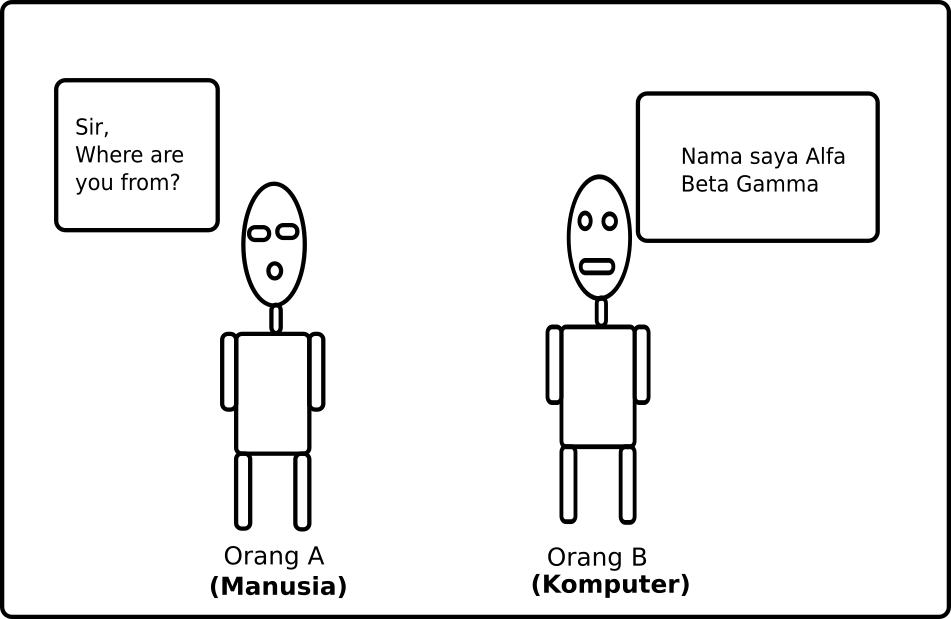
\includegraphics[width=.7\textwidth]{61_comp.png}
    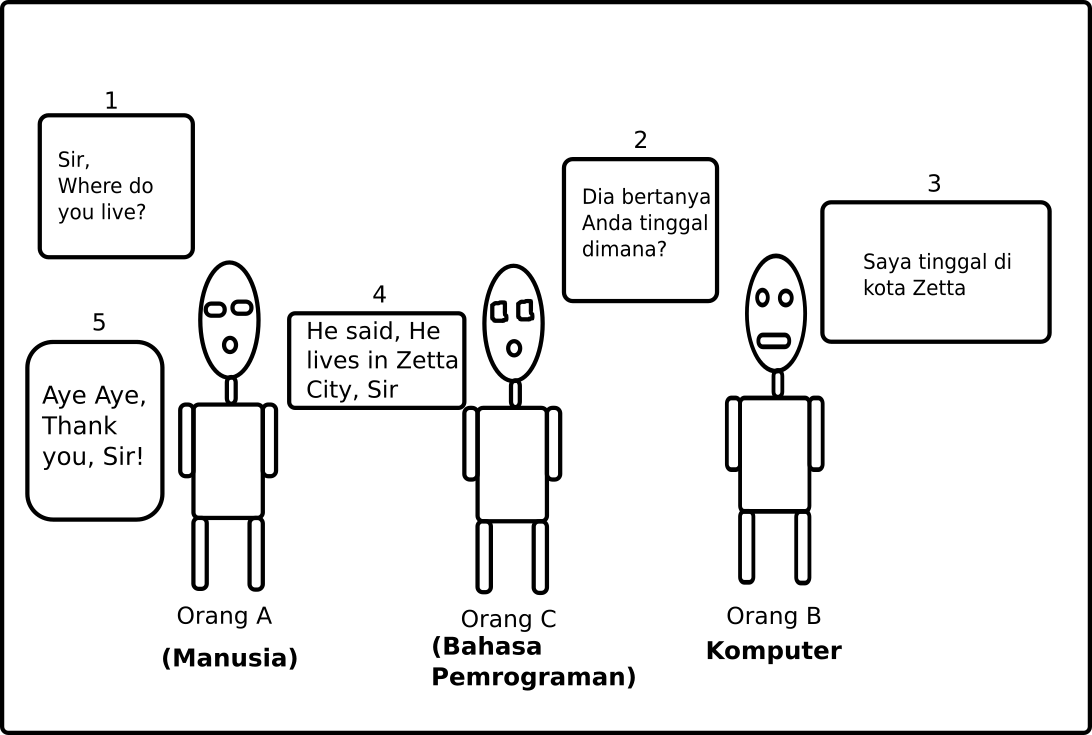
\includegraphics[width=.7\textwidth]{62_comp1.png}
    \caption{(Atas) Komunikasi 2 orang berbeda warga negara (orang A dan orang B) sebagai abstraksi komunikasi antara manusia dengan komputer. (Bawah) Komunikasi 2 orang berbeda warga negara (orang A dan orang B) kemudian ditengai oleh seorang translator (Orang C) \emph{(Gambar ini dirancang dan digambar oleh penulis)}}
    \label{fig:61_comp}
	\end{figure}

Komputer tidak bisa menulis program. Komputer juga tidak mengerti bahasa manusia. Disinilah letak peranan dari bahasa pemrograman, yaitu sebagai jembatan komunikasi antara manusia dengan komputer. Untuk abstraksi yang lebih jelas terkait dengan peranan bahasa pemrograman dapat Anda amati pada gambar (\ref{fig:61_comp}). 

Pada gambar tersebut (gambar atas) tedapat 2 orang yang berbeda warga negara (Orang A dan orang B) yang sedang mencoba berkomunikasi. Namun, karena menggunakan bahasa yang berbeda dapat dipastikan akan terjadi miskomunikasi. Permasalahan ini dapat diatasi apabila Anda bisa mengundang orang ketiga (orang C) sebagai \textit{translator} yang menghubungkan komunikasi antara orang A dan orang B. 

Kedua orang yang ingin berkomunikasi dapat dibayangkan sebagai manusia yang ingin memberikan instruksi pada komputer. Tentu saja, manusia tidak bisa secara langsung memberikan instruksi pada komputer. Itulah sebabnya bahasa pemrograman diciptakan yaitu untuk memberikan jembatan komunikasi antara manusia dan komputer. 

Dari sini bisa didefinisikan bahwa bahasa pemrograman adalah bahasa yang digunakan untuk berkomunikasi dengan komputer. Menurut tingkatannya, bahasa pemrograman dapat dibedakan menjadi 3 kategori yaitu :
\begin{itemize}
	\item Bahasa mesin
	\item Bahasa assembly
	\item Bahasa tingkat tinggi
\end{itemize}

\subsection{Bahasa Mesin}
 Pada gambar (\ref{fig:61_comp}) disebutkan bahwa mesin dibayangkan dapat berkomunikasi dengan sesama mesin dengan menggunakan suatu bahasa tertentu. Bahasa itulah yang dimaksud dengan bahasa mesin. Bahasa mesin (kode mesin) merupakan bahasa tingkat rendah yang secara langsung dikonstruksi dan hanya diperuntukan untuk mesin. Disebut "tingkat rendah" karena konfigurasi kodenya bisa berbeda-beda untuk setiap mesin/platform. Bahasa mesin terdiri atas 2 buah nilai saja : \texttt{0} dan \texttt{1} (sehingga membentuk sistem binary), yang mana biasanya membentuk kelompok byte (8 bit). Berikut adalah contoh dari pada struktur bahasa mesin :

\begin{verbatim}
    01010101 11011011 11110010
\end{verbatim}

Mempelajari bahasa mesin bisa diibaratkan seperti mempelajari bahasa manusia purba\footnote{\textit{Homo Erectus} misalnya}. Karena kebudayaan manusia purba masih rendah tentu sistem bahasa manusia purba tidak memiliki struktur bahasa yang lazim. Sehingga bahasa tersebut sangat susah untuk diartikan dan dipelajari oleh orang manusia modern\footnote{baca "kita"}. Hanya orang-orang tertentu yang bisa mengerti (mempelajari) sistem bahasa manusia purba\footnote{Sejarahwan atau Arkeolog}. 

Mirip dengan itu, bahasa mesin sangat susah untuk dipelajari. Mengapa? Karena untuk pengaplikasiannya, Anda harus mempelajari terlebih dahulu bagaimana struktur dari konstruksi mesin yang dibangun (mengingat bahasa mesin merupakan bahasa yang tergantung oleh arsitektur mesin). Selain itu, penulisan format binary tentu tidak lazim bagi orang modern seperti kita. Dibandingkan dengan jenis bahasa pemrograman yang lain, bahasa mesin memiliki beberapa kelebihan dan kekurangan.

Kelebihan dari bahasa mesin :
\begin{itemize}
	\item Cepat, karena bahasa mesin dieksekusi secara langsung oleh mesin 
	\item Penggunaan memori yang efisien
\end{itemize}

Kekurangan dari bahasa mesin :
\begin{itemize}
	\item Tidak bisa dimengerti oleh manusia (hanya terdiri dari digit \texttt{0} dan \texttt{1}).
	\item Jika terjadi kesalahan (\textit{error}) program akan susah untuk memecahkannya.
	\item Tidak ada fungsi matematika yang tersedia.
	\item Manipulasi lokasi memori dilakukan secara langsung, sehingga mmbutuhkan programer yang bisa melakukan pelacakan untuk setiap lokasi memori.
\end{itemize}

\subsection{Bahasa Assembly}
Menggunakan bahasa mesin memang memiliki kelebihan dalam hal kecepatan, namun demikian menggunakan bahasa mesin tentu saja sangat tidak mudah bagi programer karena skrip kode hanya tediri dari 2 digit bilangan saja (\texttt{0} dan \texttt{1}). Maka dari itu, programer yang ingin bekerja dalam ranah pemrograman tingkat rendah (bahasa mesin) biasanya lebih menyenangi untuk menggunakan bahasa Assembly.

Bahasa assembly pada dasarnya menggantikan bentuk digit binary (\texttt{0} dan \texttt{1}) ke dalam simbol alfanumerik \footnote{kombinasi antara huruf alfabet dan angka-angka} dengan tujuan mempermudah bentuk bahasa mesin. Contohnya adalah sebagai berikut :
\begin{verbatim}
    ADD 1,2, result
\end{verbatim}
Program di atas bertujuan untuk melakukan penjumlahan bilangan \texttt{1} dan \texttt{2} kemudian menampilkan hasilnya.

Jika bahasa mesin bisa diibaratkan sebagai bahasa manusia zaman kuno, maka bahasa assembly bisa diibaratkan sebagai bahasa Sanskerta. Bahasa Sanskerta merupakan bahasa kuno namun lebih terbarukan dibandingkan dengan bahasa yang digunakan oleh manusia purba.  Bahasa Sanskerta sudah memiliki struktur bahasa yang valid dan jelas sehingga masih "dimungkinkan" untuk dibaca dan dipelajari. Namun demikian, untuk mempelajarinya Anda harus menguasai sistem penulisan bahasa Sanskerta terlebih dahulu. Hal ini menjadi faktor ketidakpraktisan mengingat budaya kita sudah tidak menggunakan bahasa Sanskerta lagi. 

Mirip dengan itu, mengembangkan suatu perangkat lunak dengan menggunakan bahasa assembly menjadi barang yang bersifat tidak mungkin untuk dilakukan. Dibandingkan dengan jenis bahasa pemrograman yang lain, bahasa Assembly memiliki beberapa kelebihan dan kekurangan.

Kelebihan dari bahasa assembly :
\begin{itemize}
	\item Lebih mudah digunakan dibandingkan bahasa mesin.
	\item Masih tergolong bahasa tingkat rendah, sehingga kurang cocok digunakan seorang pemula.
\end{itemize}

Kekurangan dari bahasa Assembly :
\begin{itemize}
	\item Tidak ada bentuk simbolik pada lokasi memori.
	\item Masih susah untuk digunakan (khususnya orang awam).
	\item Bentuk bahasa Assembly sangat bergantung pada arsitektur dari mesin (platform) yang digunakan. 
\end{itemize}

\subsection{Bahasa Tingkat Tinggi}
Berbeda dengan kedua jenis bahasa pemrograman di atas yang termasuk golongan bahasa pemrograman tingkat rendah, sehingga untuk penggunaannya memerlukan keahlian khusus\footnote{semisal terkait dengan ilmu konstruksi mesin}, untuk kali ini akan dibahas bahasa pemrograman tingkat tinggi. Dibandingkan dengan bahasa tingkat rendah, dengan menggunakan bahasa pemrograman tingkat tinggi Anda lebih dimudahkan. Bahasa tingkat tinggi bisa diibaratkan sebagai bahasa Inggris yang biasa Anda pelajari di sekolah. Bahasa Inggris sudah terkonstruksi secara apik sehingga sangat mudah untuk dipelajari \footnote{mayoritas manusia modern menguasai bahasa inggris}.

Mirip dengan itu, bahasa tingkat tinggi dikonstruksi untuk mempermudah manusia. Penggunaan sistem pembahasaannya lebih mendekati bahasa manusia dibandingkan dengan bahasa mesin. Bahkan, dengan menggunakan bahasa tingkat tinggi, seseorang yang tidak mengerti tentang arsitektur mesin atau sistem binary bisa melakukan mengkonstruksi program (koding). Bahasa tingkat tinggi juga merupakan bahasa pemrograman yang tidak bergantung pada platform tertentu sehingga sebagai konsekuensinya program yang dihasilkan dapat dieksekusi pada mesin yang berbeda. Namun demikian, jenis bahasa pemrograman yang lebih berorientasi kepada bahasa manusia ini membutuhkan suatu penerjemah, agar instruksi yang diberikan oleh manusia bisa dieksekusi oleh komputer. Penerjemah tersebut dapat dilakukan oleh compiler atau interpreter (tergantung dari jenis bahasa pemrogramannya). Dibandingkan dengan jenis bahasa pemrograman yang lain, bahasa tingkat tinggi memiliki beberapa kelebihan dan kekurangan.

Kekurangan dari bahasa tingkat tinggi :
\begin{itemize}
	\item Harus tersedia penerjemah (compiler atau interpreter).
	\item Kecepatan eksekusi lebih rendah jika dibandingan degan bahasa mesin dan bahasa assembly.
\end{itemize}

Kelebihan dari bahasa tingkat tinggi adalah :
\begin{itemize}
	\item Mudah digunakan (biasanya menggunakan Inggris).
	\item Dapat digunakan di berbagai mesin.
	\item Cocok untuk pemula yang memulai belajar bahasa pemrograman.
\end{itemize}

Contoh dari bahasa tingkat tinggi antara lain adalah C, C++, C#, Java, Fortran, Ruby, Perl, Python dlsb. Bahasa pemrograman tersebut dikonstruksi berdasarkan filosofi dan tujuan komputasi tertentu.

\section{Mengapa harus Python?}
Dewasa ini, Python menjadi bahasa pemrograman yang paling ingin dikuasai oleh mayoritas semua orang (terutama dari kalangan programer). Antusiasme tersebut didukung oleh pesatnya perkembangan teknologi Data Sains \footnote{Data Sains adalah ilmu yang mempelajari perilaku data, baik itu data kuantitatif ataupun numerik.}. Pada bidang Data Sains, dibandingkan dengan bahasa pemrograman lainnya, Python memiliki keunggulan tersendiri dalam hal analitik karena tersedianya library NumPy, Pandas dan Matplotlib (sebagai visualisasi data).

Berbicara terkait library, kini telah tersedia berjuta-juta library di Python. Hal tersebut tentu saja akan mempermudah pekerjaan Anda karena Anda tidak diwajibkan lagi untuk membuat program dari awal. Untuk menuliskan program tertentu Anda hanya perlu memanggil fungsi dari suatu library kemudian menerapkan fungsi tersebut ke dalam program yang sedang Anda kembangkan.

Selain itu, Python sangat mudah untuk dipelajari. Jika Anda belum pernah menginjakan kaki di dunia IT (pemrograman khususnya) maka Python merupakan langkah awal yang tepat. Python juga sangat cocok untuk digunakan sebagai media pembelajaran bahasa pemrograman di dunia pendidikan mengingat Python termasuk bahasa pemrograman yang bersifat \textit{open source}. Meskipun Python merupakan bahasa pemrograman yang mudah dipelajari, Python tetap bisa untuk dijadikan basis untuk membangun sistem yang kompleks.

Satu hal lagi yang membuat Python disenangi oleh kalangan penggiat IT. Python memiliki komunitas yang luas. Jika saja Anda mengalami kesulitan belajar, selalu mengalami kesalahan (\texit{error}) dalam pengembangan program Anda, Anda bisa mengunjungi komunitas Python di forum online yang tersebar luas di internet. Contohnya Anda bisa mengunjungi website : \url{https://www.python.org/community/} dan \url{https://www.stackoverflow.com}.

\section{Soal Latihan}
\begin{enumerate}
	\item Buatlah Essay dengan tema "mengapa belajar pemrograman itu penting"!
	\item Di dalam bahasa pemrograman tingkat tinggi terdapat beberapa paradigma (sudut pandang) dalam  penyajian pemecahan masalah. Diantaranya adalah pemrograman \textit{Imperative}, \textit{Logical}, \textit{Functional} dan \textit{Object-Oriented}. Jelaskan perbedaan dari keempat paradigma pemrograman berikut!
	\item Di dalam bahasa tingkat tinggi terdapat 2 jenis penerjemah, Compiler dan Intrepreter. Jelaskan bagaimana 2 penerjemah itu bekerja kemudian bandingkan juga kekurangan dan kelebihannya!
	\item Sebutkan kelebihan dan kekurangan bahasa pemrograman Python dibandingkan bahasa pemrograman yang lainnya!
	\item Jelaskan bagaimana pembuatan alur program sehingga program tersebut dapat digunakan untuk memecahkan suatu masalah?
\end{enumerate}

%----------------------------------------------------------------------------------------
%	CHAPTER 2: Dasar Pemrograman
%----------------------------------------------------------------------------------------
%\chapterimage{head1.png}

\chapter{VISUALISASI DATA}
\section{Apa itu Data?}
Data adalah representasi nyata dari suatu objek. Data dapat berbentuk teks, numerik, gambar (warna), suara, dlsb.

\section{Fungsi Data}
\begin{enumerate}
	\item Sebagai acuan untuk melakukan pengkajian.
	\item Sumber kajian dan evaluasi dari suatu aktivitas.
	\item Acuan dalam menentukan kebijakan/keputusan untuk kedepannya.
\end{enumerate}

\section{Jenis Data}
Pada dasarnya data dapat dibedakan menjadi 2 :
\begin{enumerate}
	\item Data Kualitatif
	\item Data Kuantitatif
\end{enumerate}

\subsection{Data Kualitatif}
Data kualitatif merupakan representasi obyek yang berbentuk pernyataan kwalitas. Biasanya data kualitatif diformasi dari rekam pendapat yang sifatnya \textbf{subyektif}. Artinya, bisa saja antara 2 orang yang berbeda dapat memberikan pemberian data yang berbeda dalam 1 obyek yang sama.

Semisal terdefinisi seekor sapi. Sapi tersebut memilki data kualitatif sebagai berikut.
\begin{table}[hbt!]
  \centering
   \caption{Data kualitatif pada sapi}
   \label{tab:1-1}
  \begin{tabular}{ p{3cm} p{7cm} }
    \hline\hline
    Data & Deskripsi\\
    \hline
    Keadaan & Sehat \\
    Warna & Hitam-putih \\
    Tekstur & Lembut \\
    \hline 
  \end{tabular}
\end{table}

Adapun metode pengumpulan data adalah sebagai berikut.
\begin{enumerate}
	\item Pertanyaan (wawancara)
	\item Diskusi
	\item Observasi
\end{enumerate}

Analisa data kualitatif.
Tidak ada aturan yang pasti terkait dengan metode analisa pada data kualitatif. Mengapa? Hal tersebut dikarenakan data dianggap sesuatu yang telah benar (subyektif). Adapun metode yang sering kali digunakan adalah sebagai berikut :
\begin{enumerate}
	\item Pendekatan Deduktif 
	Strukur penelitian ditentukan oleh peniliti. Cepat dan Mudah.
	\item Pendekatan Induktif
	Pendekatan ini tidak secara langsung ditentukan oleh peneliti. Lama dan susah.
\end{enumerate}

\subsection{Data Kuantitatif}
Data kuantitatif adalah data yang bisa direpresentasikan dalam bentuk angka-angka (nilai numerik). Data kuantitatif dapat dihasilkan dari suatu eksperimen (pengukuran maupun observasi). Data kuantitatif relatif lebih bersifat obyektif karena didapatkan dari hasil pengukuran bukan dari pendapat seseroang. 

Semisal terdefinisi seekor sapi. Sapi tersebut memilki data kualitatif sebagai berikut.
\begin{table}[hbt!]
  \centering
   \caption{Data kuantiatif pada sapi}
   \label{tab:1-1}
  \begin{tabular}{ p{3cm} p{7cm} }
    \hline\hline
    Data & Deskripsi\\
    \hline
    Berat & 300 kg \\
    Panjang & 3 meter \\
    Harga & 16.000.000 \\
    \hline 
  \end{tabular}
\end{table}

Adapun metode pengumpulan data adalah sebagai berikut.
\begin{enumerate}
	\item Pertanyaan (wawancara)
	\item Sampling probabilitas
	\item Survei atau kuesioner
	\item Pengamatan
\end{enumerate}

Analisa data kuantitatif :
\begin{enumerate}
	\item Analisa Maxdiff 
	\item Tabulasi Silang
	\item Analisa SWOT
\end{enumerate}

Langkah analisa data kuantitatif:
\begin{enumerate}
	\item Hubungkan skala pengukuran dengan variabel
	\item Hubungkan statistif dekskriptif dengan data
	\item Tentukan skala pengukuran 
	\item Pemilihan tabel 
\end{enumerate}

\section{Data Diskrit vs Data Kontinyu}
Dari perilaku datanya data dapat dibedakan menjadi 2 :
\begin{enumerate}
	\item Data diskrit
	\item Data kontinyu
\end{enumerate}

\subsection{Data Diskrit}
Data diskrit merupakan data yang terkumpul hasil dari pencacahan. Contoh data jumlah kehadiran  orang dalam suatu acara atau jumlah peliharaan ayam Anda di kandang. Pada data diskrit Anda tidak mungkin mendapatkan nilai desimal, Anda tidak mungkin menghitung kehadiran pada suatu kelompok dengan jumlah 11.5 orang.

Adapun karakteristik dari data diskrit adalah sebagai berikut :
\begin{enumerate}
	\item Dapat dihitung
	\item Nilai tidak mungkin menjadi desimal (pecahan)
	\item Tidak dapat diukur (menggunakan alat)
	\item Biasanya direpresentasikan dalam bentuk grafik batang
\end{enumerate}

\subsection{Data Kontinyu}
Data kontinyu merupakan data yang terkumpul dari hasil perhitungan. Semisal Anda ingin mengetahui panjang dari suatu meja. Anda akan mengukurnya menggunakan mistar bukan mencacahnya bukan? Hasil yang didapatkan pun bisa berbentuk desimal (pecahan), mungkin panjang dari meja Anda dapat bernilai 100.5 cm,

Adapun karakteristik dari data kontinyu adalah sebagai berikut :
\begin{enumerate}
	\item Dapat diukur (menggunakan alat)
	\item Nilai mungkin menjadi desimal (pecahan)
	\item Tidak dapat dicacah
	\item Biasanya direpresentasikan dalam bentuk grafik histogram
\end{enumerate}

\section{Data Numerik vs Data Kategori}
Data juga dapat dibedakan berdasarkan nilai variabelnya, yaitu:
\begin{enumerate}
	\item Data Numerik
	\item Data Kategori
\end{enumerate}

\subsection{Data Numerik}
Data yang identik dengan nilai numerik. Data numerik dapat dibedakan menjadi data diskrit dan kontinyu.

\subsection{Data Kategori}
Data yang bisa dikategorikan berdasarkan karaketeristik masing-masing individu data. Contohnya status perkawinan data di KTP, agama, kota asal, hobi, jenis kelamin dlsb.
\subsubsection{Data Nominal}
Data nominal merupakan data yang tidak memiliki korelasi atau kerterkaitan dengan data lainnya. Contoh : jenis kelamin, pekerjaan dlsb.

Ciri-ciri data nominal :
\begin{enumerate}
	\item Hasil pencacahan (tidak dalam bentuk desimal)
	\item Angka yang mucnul hanya digunakan sebagai penera (simbol)
	\item Simbol dapat berbentuk angka, huruf, lambang dlsb.
\end{enumerate}

\subsubsection{Data Ordinal}
Data ordinal merupakan suatu bilangan diskrit yang memiliki derajat urutan tertentu. Contohnya waktu yang muncul sebagai rangking orang berlari. Orang A : 1 jam, Orang B : 1 jam 10 menit, orang C : 1 jam 11 menit dlsb.

\section{Data Terstrukur vs Data Tidak Terstruktur}
\subsection{Data Terstruktur}
Biasanya terformat dalam tabel. Contohnya data excel, data RDBMS, kartu stok dlsb.
\subsection{Data Tidak Terstruktur}
Lebih beragam bentuknya. Contohnya citra image pada satelit, noise dari sadap, dlsb.
\subsection{Data Semi Terstruktur}
XML, file .csv, JSON dlsb.

\section{Visualisasi Data}
Cara mengkomunasikan data dengan format visual tertentu, semisal diagram, grafik atau representasi lainnya. 

Tujuan visualisasi data :
\begin{enumeraate}
	\item Komunakasi lebih efektif.
	\item Pemantauan data lebih mudah.
\end{enumerate}

Media visualisasi data :
\begin{enumeraate}
	\item Tabel. 
	Perhatikan : Judul, kesederhaan, penjelasan simbol, penekanan pada suatu data tertentu, sumber tabel.
	\item Diagram.
	Jenis : diagram batang, diagram garis, diagram lingkaran.
\end{enumerate}

%copas
Visualisasi Data dalam bisnis :
\begin{enumeraate}
	\item Dashboard.
	Dashboard merupakan kumpulan dari berbagai visualisasi yang berbeda yang menggabungkan dan merangkum informasi atau data bisnis. 
	\item Scoreboard
	Scorecard merupakan tipe lainnya dalam visualisasi di bidang bisnis. Berbeda dengan dashboard yang terdapat banyak visualisasi di dalamnya, scorecard lebih fokus pada sebuah target tertentu. Visualisasinya berupa  jumlah pendapatan, kepuasan pelanggan, dan hal lainnya yang dapat dibandingkan dengan target yang telah ditentukan. Scorecard juga biasanya disajikan dalam salah satu komponen dashboard. Scorecard menggambarkan tentang Key Performance Indicators (KPI) yang lebih disederhanakan untuk dapat memantau kemajuan progres.
	\item Analytic report
	Analytic report atau laporan yang berisi analisis yang digunakan untuk menentukan keputusan. Jenis laporan ini menggunakan data kualitatif dan kuantitatif untuk menganalisis dan mengevaluasi ide dari suatu bisnis. Analytic report memberikan keuntungan untuk pembaca karena memberi  pemahaman yang mudah dipahami. Selain itu hanya dengan membaca sekilas saja. pembaca juga dapat memahami data dalam jumlah yang banyak. 

	Analytic report juga menerapkan langkah-langkah umum seperti mengidentifikasi masalah, menentukan metode yang tepat, analisis data, dan mendapatkan solusi terbaik dari masalah yang dihadapi.
	\item Report
	Report merupakan bagian dari visualisasi data dalam bisnis yang memuat semua ringkasan dari apa yang terjadi di perusahaan dalam waktu tertentu. Inti dari report adalah apa yang Anda lakukan untuk mendapatkan dan memahami hal yang sedang terjadi dari suatu perusahaan dengan secepat mungkin.
\end{enumerate}

Tool yang bisa Anda gunakan :
\begin{enumeraate}
	\item Tableau Public
	Tableau Public merupakan sebuah layanan gratis yang memungkinkan siapa saja dapat mempublikasikan visualisasi data ke dalam web. Visualisasi yang telah dipublikasikan ke Tableau Public ("vizzes") dapat diletakkan dalam halaman web dan blog, dibagikan ke sosial media, dan juga dapat juga diunduh oleh pengguna lainnya. Untuk proses pembuatan visualisasi datanya sendiri menggunakan aplikasi terpisah bernama Tableau Desktop Public Edition. Ingin tahu hal yang menarik dari Tableau Desktop Public ini? Ya, Anda dapat menggunakan aplikasi ini tanpa memerlukan keahlian dalam bidang pemrograman. Keren, bukan? Untuk mengunduh aplikasi Tableau Public dapat klik di sini, ya.
	\item Google Sheets
	Sudah pernah menggunakan Google Sheets sebelumnya? Anda tidak harus melakukan instalasi aplikasi spreadsheet di laptop Anda, karena dalam Google Spreadsheet semuanya tersedia online. Google Sheets menawarkan kumpulan fitur dan fungsi standar spreadsheet application seperti yang ada di Microsoft Excel. Tentunya pada Google Sheets dapat membuat visualisasi sederhana dari data yang kita buat baik dalam bentuk diagram batang, diagram garis, maupun diagram lingkaran.
	\item Microsoft Excel
	Pasti Anda familiar dengan Microsoft Excel, bukan? Sebuah aplikasi spreadsheet buatan Microsoft yang memuat banyak fitur powerful. Microsoft Excel menggunakan spreadsheet yang terdiri dari baris dan kolom untuk manajemen data serta melakukan perhitungan fungsi yang lebih akrab disebut formula. Selain melakukan perhitungan angka yang bersifat numerik, Excel juga dapat membuat visualisasi data sederhana ke dalam bentuk grafik seperti diagram garis, batang, lingkaran, dan lain-lain.
\end{enumerate}

%\input{bab/14_parsial}
\appendix
\chapter{GLOSARIUM}
\textbf{Algoritma} Tata cara untuk menyelesaikan masalah secara sistematis.\\ \\
\textbf{Assembly}  Bahasa pemrograman tingkat rendah (satu tingkat di atas bahasa mesin) yang sangat bergantung pada arsitektur mesin tertentu. \\ \\
\textbf{Array}  Variabel yang dapat menampung nilai lebih dari satu namun harus memiliiki tipe data yang sama. \\ \\
\textbf{Compiler} Suatu program khusus yang digunakan untuk mengeksekusi instruksi pada suatu skrip program dengan melakukan kompilasi (penerjemahan pada bahasa tertentu, contohnya bahasa mesin). \\ \\
\textbf{Dict} Salah satu struktur data pada Python yang merupakan variabel multinilai yang komponen nilainya berupa kunci dan nilai (seperti kamus). \\ \\
\textbf{Fungsi} Kumpulan instruksi program yang memiliki sebuah tujuan tertentu. \\ \\
\textbf{IDE} Kepanjangan dari Integrated Development Environtment yaitu gabungan (kesatuan) dari pada interpreter/compiler, library, text-editor, debugging, dlsb yang dikonstruksi untuk memudahkan pengembangan suatu program.\\ \\
\textbf{Interpreter} Suatu program khusus yang digunakan untuk mengeksekusi instruksi pada suatu skrip program tanpa melakukan kompilasi.\\ \\
\textbf{Indentasi} Blok pada program Python yang dicirikan dengan tulisan yang lebih menjorok (hasil eksekusi tombo "tab"). \\
\textbf{Kelas} Cetak biru dari objek.\\ \\
\textbf{Konstanta} Wadah dari suatu nilai namun nilainya tidak berubah.\\ \\
\textbf{Konstruktor} Method khusus yang digunakan untuk memberikan keadaan awal dari suatu objek sejak objek tersebut diinstanisasi (diwujudkan).\\ \\
\textbf{Konvergen} Keadaan dimana hasil iteratif dari suatu perhitungan menuju pada suatu nilai tunggal.\\ \\
\textbf{List} Salah satu struktur data pada Python yang merupakan variabel multinilai yang komponen nilainya bisa berubah.\\ \\
\textbf{Numpy} Salah satu library pada Python yang digunakan untuk komputasi ilmiah berbasis array.\\ \\
\textbf{Matplotlib} Salah satu library pada Python yang digunakan untuk visualisasi data.\\ \\
\textbf{Matriks} Sebuah entitas matematika dimana datanya diatur sedemikian rupa menjadi deret dan kolom.\\ \\
\textbf{Objek} Representasi atau pemodelan "sesuatu" yang eksis di dunia nyata untuk mewadahi suatu atribut (data) dan perilaku (method) dari suatu sistem tertentu.\\ \\
\textbf{Operator} Simbolisme dari suatu perintah manusia kepada komputer (melalui intepreter atau compiler) untuk melakukan suatu operasi khusus seperti operasi aritmatika, operasi logika, operasi relasi, dlsb.\\ \\
\textbf{Jupyter Notebook} Salah satu IDE untuk bahasa Python berbasis web.\\ \\
\textbf{Polimorpisme} Fitur dari paradigma objek yang mengizinkan Anda untuk mengimplementasikan varibel dan method yang sama pada anak kelas dengan cara yang berbeda.\\ \\
\textbf{Program} Kumpulan instruksi untuk melaksanakan suatu tugas tertentu.\\ \\
\textbf{Programer} Seseorang yang memiliki kapabilitas untuk menkonstruksi program untuk menyelesaikan suatu masalah tertentu.\\ \\
\textbf{Pycharm} Salah satu IDE untuk bahasa Python berbasis dekstop.\\ \\
\textbf{Python} Salah satu jenis pemrograman tingkat tinggi yang menggunakan interpreter dengan fitur dynamic-binding dan dynamic-typing.\\ \\
\textbf{Tipe data} Klasifikasi data berdasarkan perilakunya (ukuran data, pengoperasiannya, dlsb)\\ \\
\textbf{Rekursif} Jenis fungsi yang digunakan untuk melaksanakan prinsip pengulangan dengan jalan memanggil dirinya sendiri.\\ \\
\textbf{RPEL} Kepanjangan dari Read Evaluate Print Loop yaitu interaktif interpreter (biasanya berupa tampilan Command Line Interface).\\ \\
\textbf{Sistem Linear} Sistem persamaan yang suku variabel independennya terbatas memiliki derajat pangkat satu.\\ \\
\textbf{Sistem Nonlinear} Sistem persamaan yang suku variabel independennya memiliki derajat pangkat lebih dari satu.\\ \\
\textbf{Set} Salah satu struktur data pada Python yang merupakan variabel multinilai yang komponen nilainya bersifat unik.\\ \\
\textbf{Sistem Operasi} Program (perangkat lunak) yang bertanggung jawab melakukan manajemen kinerja antara perangkat keras dengan perangkat lunak lainnya.\\ \\
\textbf{Tuple} Salah satu struktur data pada Python yang merupakan variabel multinilai yang komponen nilainya tidak bisa berubah.\\ \\
\textbf{Variabel} Wadah dari suatu nilai yang berada di dalam memori RAM.\\ \\


\begin{thebibliography}{99}
		\chapterimage{head1.png} % Table of contents heading image
		\pagestyle{empty} % No headers
		\pagestyle{fancy} % Print headers again  

		\bibitem[Boas, M.L. (2005)] {boas} Boas, M.L. 2005. \textit{Mathematical Methods in The Physical Sciences}. Canada: John Wiley \& Sons, Inc. 	%sudah_tersitasi

		\bibitem[Burden, R.L. dan Faires, J.D (2010)] {burden} Burden, R.L. dan Faires, J.D. 2010. \textit{Numerical Analysis, Ninth Edition}. Canada: Cengange Learning. %sudah_tersitasi

		\bibitem[Cooper, J. (2001)] {cooper} Cooper, J. 2001. \textit{A MatLab Companion for Multivariable Calculus}. San Diego: Harcour Academic Press. 
		%sudah_tersitasi

		\bibitem[Esfandiari, R.S. (2017)] {esfandiari} Esfandiari, R.S. 2017. \textit{Numerical Methods for Engineers and Scientists Using MATLAB, Second Edition}. Florida: CRC Press.
		%sudah_tersitasi

		\bibitem[Goodrich, M.T., dkk.(2013)] {goodrich} Goodrich, M.T., Tamassia, R. dan Goldwasser, M.H. 2013. \textit{Data Structures and Algorithms in Python}. Florida: John Wiley \& Sons, Inc.
		%sudah_tersitasi	

		\bibitem[Gowrishankar, S. dan Veena, A. (2019)] {veena} Gowrishankar, S. dan Veena, A. 2019. \textit{Introduction to Python Programming}. Florida: CRC Press. 
		%sudah_tersitasi

		\bibitem[Kiusalaas (2005)] {kiusalaas} Kiusalaas, J. 2005. \textit{Numerical Methods in Engineering with Python}. New York: Cambridge University Press.
		%sudah_tersitasi

		\bibitem[Landau, R.H., dkk. (2015)] {landau} Landau, R.H., Paez, M.J. dan Bordeianu, C.C. 2015. \textit{Computational Physics: Problem Solving with Python}. Weinheim: Wiley-VCH.%sudah_tersitasi

		\bibitem[Mueller, J.P. (2018)] {mueller} Mueller, J.P. 2018. \textit{Beginning Programming with Python for Dummies, Second Edition}. Canada: John Wiley \& Sons, Inc.
		%sudah_tersitasi

		\bibitem[Nagar, S. (2018)] {nagar} Nagar, S. 2018. \textit{Introduction to Python for Engineers and Scientists: Open Source Solutions for Numerical Computation}. New York: Apress. %sudah_tersitasi

		\bibitem[Nelli, P. (2018)] {nelli} Nelli, P. 2018. \textit{Python Data Analytics: with Pandas, NumPy and Matplotlib, Second Edition}. New York: Apress. 
		%sudah_tersitasi

		\bibitem[Pine, D.J. (2019)] {pine} Pine, D.J. 2019. \textit{Introduction to Python for Science and Engineering}. Boca Raton: CRC Press. %sudah_tersitasi

		\bibitem[Riley, K.F., dkk (2006)] {riley} Riley, K. F., Hobson, M.P. dan Bence, J.C. 2006. \textit{Mathematical Methods for Physics and Engineering}. New York: Cambridge University Press.%sudah_tersitasi


		\bibitem[Solomon, J. (2005)] {solomon} Solomon, J. 2015. \textit{Numerical Algorithms: Methods for Computer Vision, Machine Learning and Graphics}. Florida: CRC Press.%sudah_tersitasi

		%Web :
		\bibitem[\url{jetbrains.com} (2019)]{jecbrains.com}\url{https://www.jetbrains.com/pycharm/}. Diakses tanggal 24 Desember 2019, pukul 06.06 WIB. %sudah_tersitasi

		\bibitem[\url{python.org} (2019)]{python.org}\url{https://www.python.org/community/}. Diakses tanggal 24 Desember 2019, pukul 11.06 WIB.%sudah_tersitasi

		\bibitem[\url{stackoverflow.org} (2019)]{stackoverflow.com}\url{https://www.stackoverflow.com}. Diakses tanggal 25 Desember 2019, pukul 14.06 WIB.%sudah_tersitasi

\end{thebibliography}
\printindex
\end{document}